As mentioned in \ref{sec:Introduction:Problem Definition}, our solution must be capable of both designing a feasible trajectory for each of the robots capable of transporting the payload and creating an adaptive control law to be used by the robots during the execution of the trajectory. The system architecture we are proposing is depicted in \ref{fig:Proposed Approach: System Architecture : System Architecture}. Unlike the classical approach to path and trajectory planning, our approach introduces a closed-loop system, described as a continuous planning system, as explained in~\cite{durfee1999survey}. This method is suitable for scenarios where the environment can undergo changes caused by unknown agents. 

The primary advantage of incorporating a feedback loop not only in the control phase but also in the trajectory generation phase is its ability to adapt and correct model errors. Additionally, it enables payload transportation even in the absence of information about mechanical parameters, resulting in a robust system capable of functioning in diverse scenarios. This robustness cannot be achieved with classical planning approaches, where the generated trajectory is not reassessed during execution.

\begin{figure}[H]
    \centering
    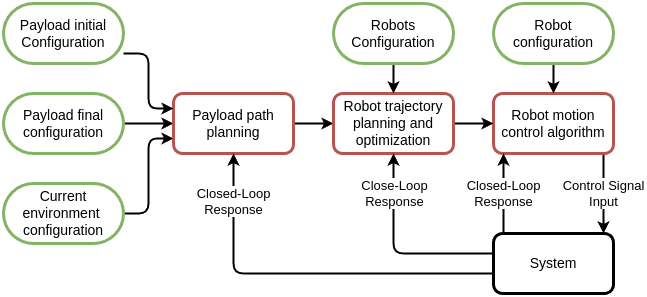
\includegraphics[width=0.7\textwidth]{Images/Propposed Aproach/System Architecture.png}
    \caption{System Architecture}
    \label{fig:Proposed Approach: System Architecture : System Architecture}
\end{figure}

The feedback loops can be managed in two distinct ways: fixed time step or event-driven. In the fixed time step approach, the system checks whether the trajectory needs replanning after a predefined time interval. If replanning is required, the corresponding module updates the trajectory, and the system begins using the new reference. In the event-driven approach, trajectory replanning is triggered by specific events, such as obstacle detection or a drift between the reference and the actual position. 

Both methods have advantages, but certain constraints must be met. If a previous stage utilizes a fixed time step, all subsequent stages must also follow a fixed time step. Additionally, the control algorithm always operates on a fixed time step. This results in the possibilities presented in \ref{tab:Proposed Approach: System Architechture}. The final configuration will be defined in the final report after additional testing to determine the optimal approach and establish a baseline for comparison.

\begin{table}[H]
    \centering
    \resizebox{0.8\textwidth}{!}{%
    \begin{tabular}{ccc}
    \hline
        \textbf{} & \textbf{Payload Path Planning} & \textbf{Robots Trajectory Planning} \\ \hline
        \textbf{Scenario 1} & Event-Driven & Event-Driven \\ 
        \textbf{Scenario 2} & Event-Driven & Fixed Rate \\ 
        \textbf{Scenario 3} & Fixed Rate & Fixed Rate \\ \hline
    \end{tabular}
    }
    \caption{Multiple allowed feedback architectures}
    \label{tab:Proposed Approach: System Architechture}
\end{table}
